Located at one of the four intersections of the LHC beams, the CMS detector is designed to measure the resulting collisions to high precision~\cite{CMS}. It's key features are the precise determination of the properties of single particles as well as a good coverage of the 4$\pi$ solid angle. The central element of the CMS detector is a superconducting solenoid. Cooled to $\unit{4.45}{\kelvin}$, it is able to produce a homogeneous magnetic field of $\unit{3.8}{\tesla}$, which allows to measure the momentum of charged particle by bending their trajectories. As shown in Figure~\ref{fig:CMS}, the different components of the detector are layered in cylindrical shapes around the interaction point. The magnet encompasses most of the main subdetectors, namely the tracking system which measures the trajectories of charged particles and the electromagnetic and hadron calorimeters, designed to measure the energy of particles. Located outside of the volume of the solenoid are the iron return yoke and muon detectors. This cylindrical structure is complemented on both sides by endcaps, which close the solid angle in the direction of the beams and are partly located outside the volume of the solenoid. The different components are described in more detail in the following. 
\begin{figure}[htbp]
\centering
  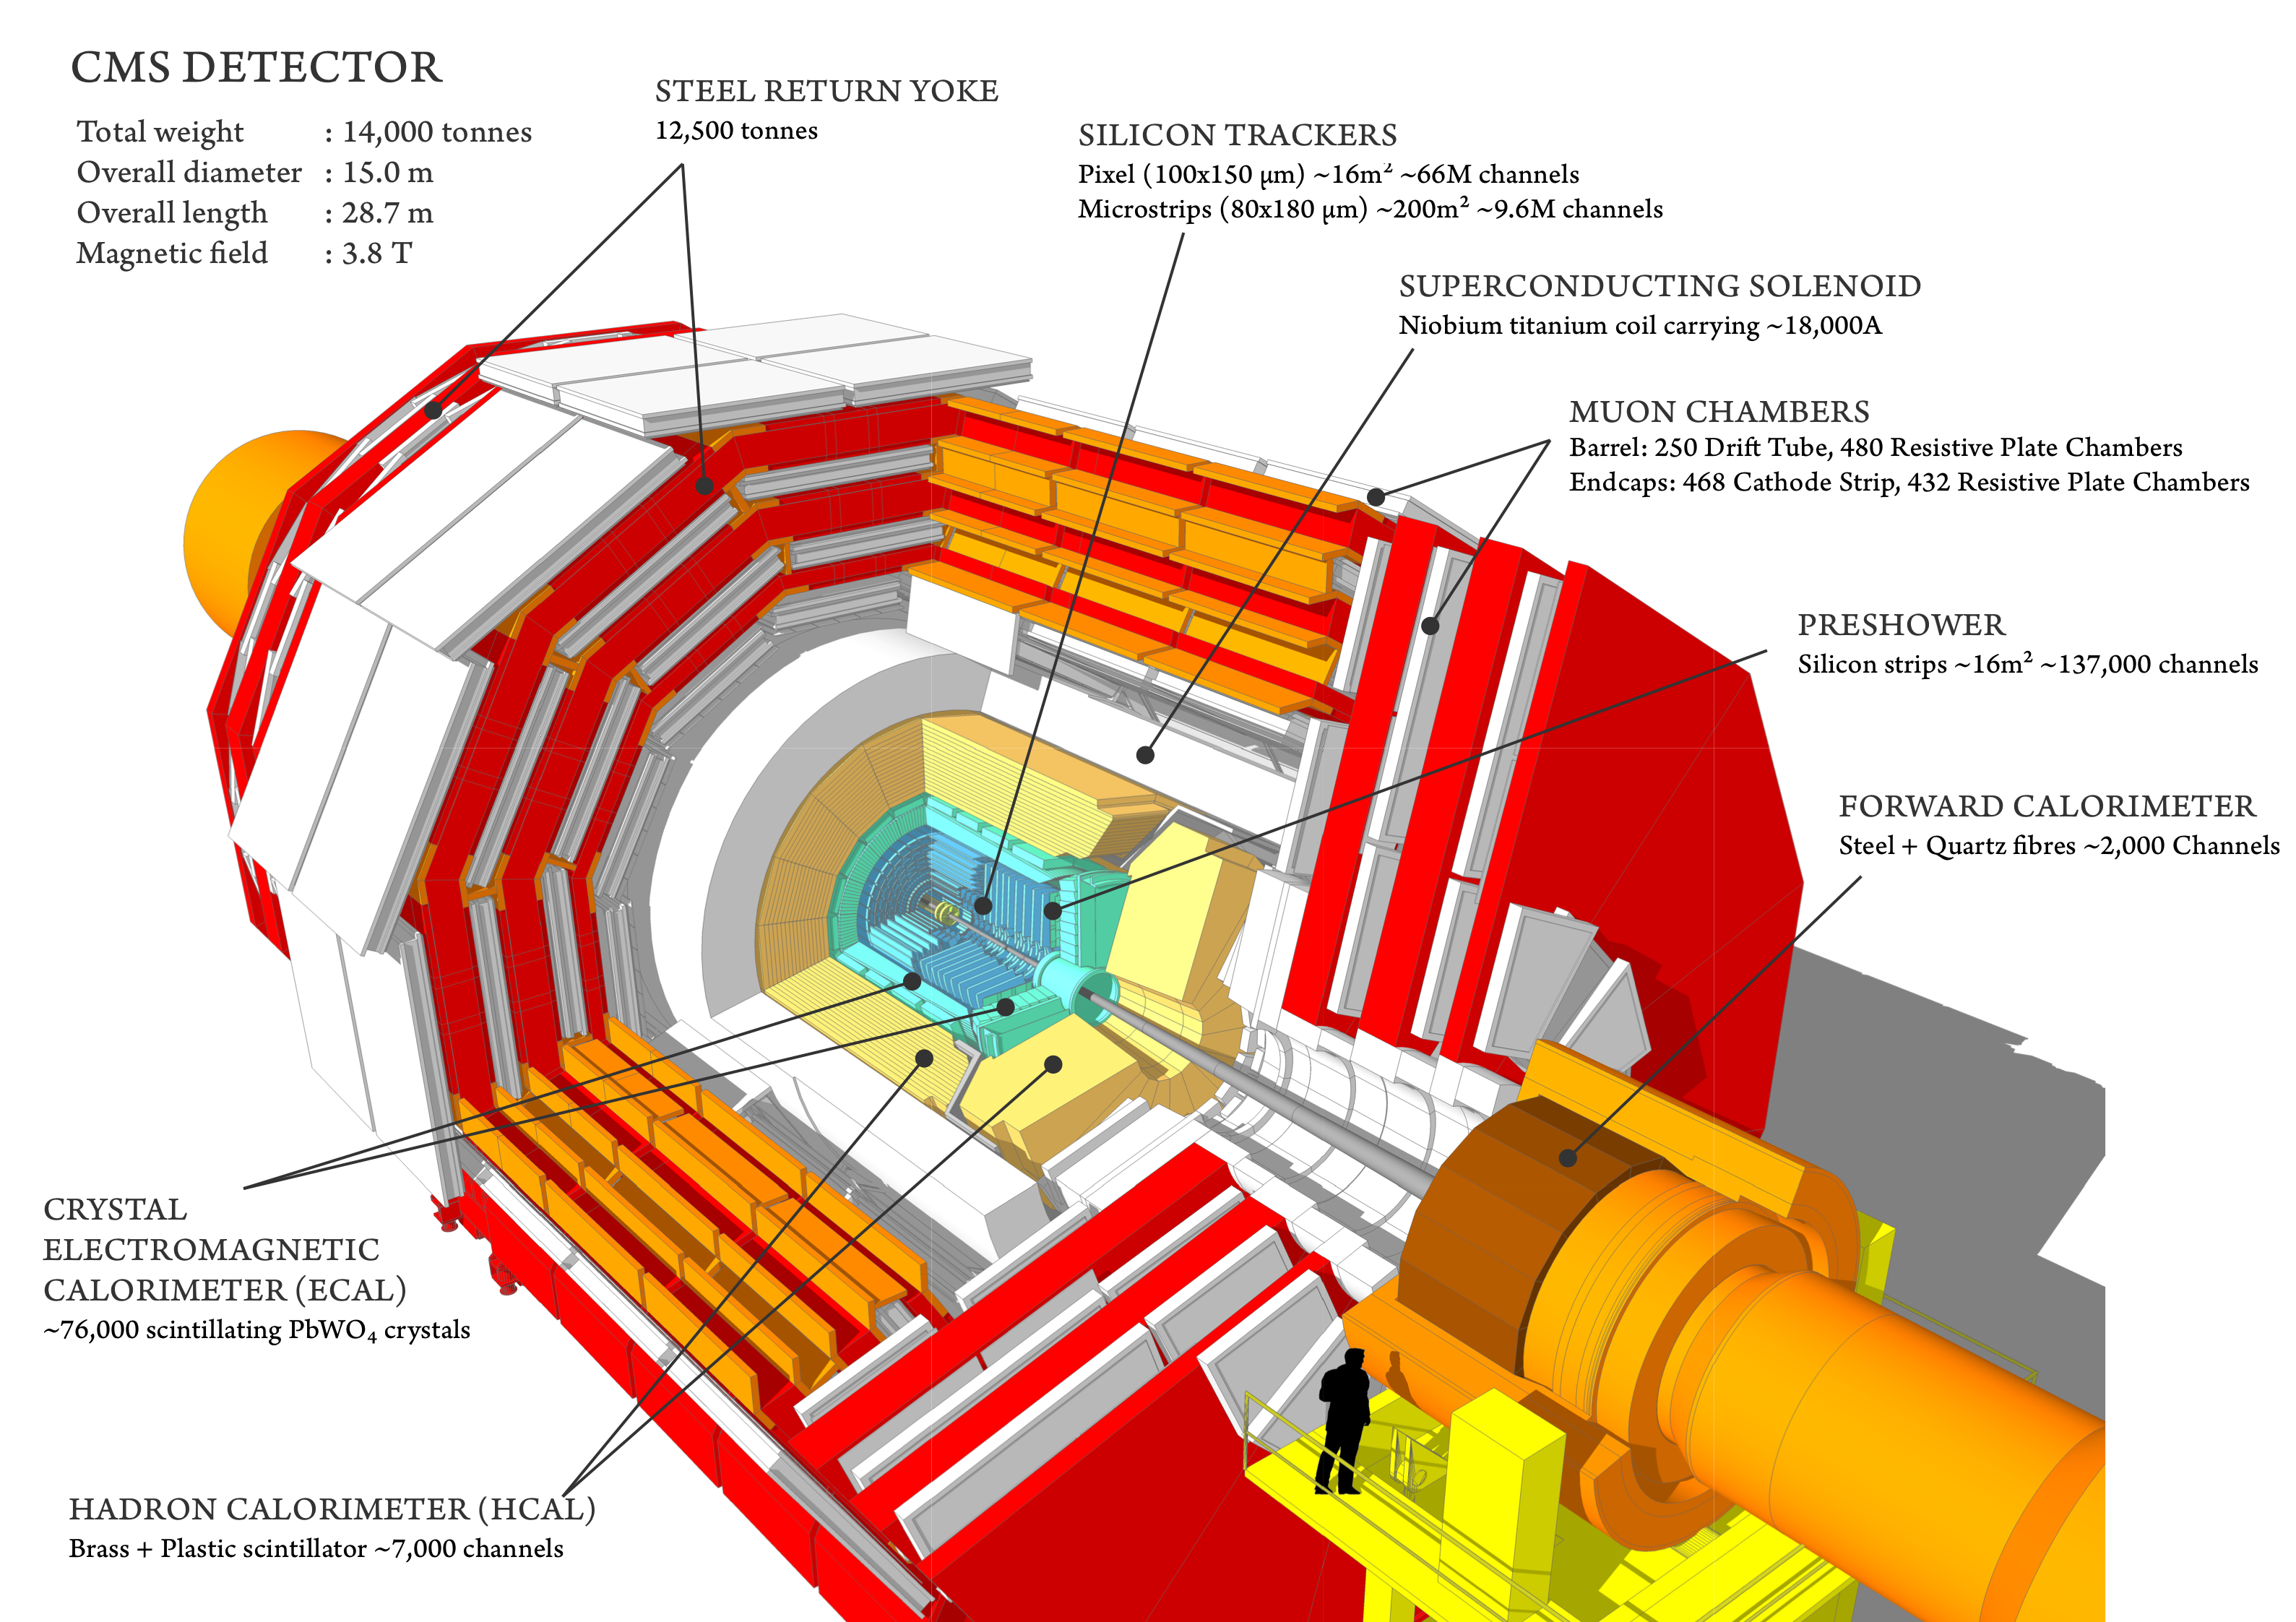
\includegraphics[width=0.8\textwidth]{plots/CMS/cms_design.png}
\caption{Schematic view of the CMS detector~\cite{CMSScetch}. From the inside out, the tracking system is shown in blue, the electromagnetic calorimeter in green, the hadron calorimeter in light yellow, the superconducting solenoid in white, the return yoke in red, and the muon system again in white.}
\label{fig:CMS}
\end{figure}
\subsection{Tracking system}
The tracking system of the CMS detector consists of many layers of silicon pixels and strips. The trajectories of charged particles are reconstructed from the ionisation signal they cause in the silicon. In the magnetic field these trajectories bend, allowing to determine the momentum of particles. The tracking system has a diameter of $\unit{2.5}{\meter}$ and a length of $\unit{5.8}{\meter}$, corresponding to a geometric coverage of $\vert \eta \vert < $ 2.5. The tracking detector consists, as shown in Figure~\ref{fig:tracker}, of the pixel detector (PIXEL) surrounded by various components of  the silicon strip tracker. 
\begin{figure}[htbp]
\centering
  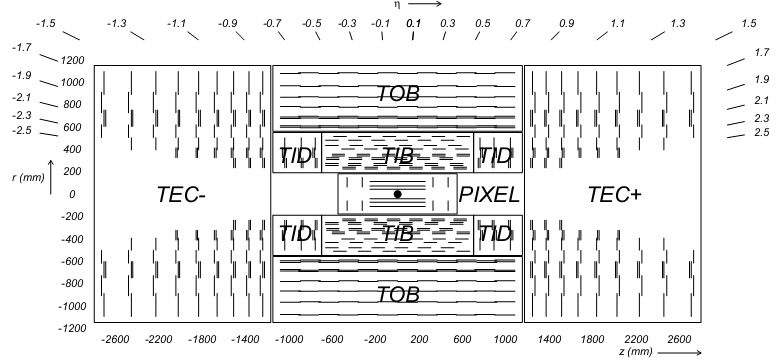
\includegraphics[width=0.85\textwidth]{plots/CMS/Tracker.png}
\caption{Schematic view of the CMS tracking detector. The innermost part shows the pixel detector (PIXEL), surrounded by the tracker inner barrel (TIB) and tracker inner discs (TID). The outermost parts of the tracking detector are the tracker outer barrel (TOB) and the two tracker endcaps (TEC+ and TEC-)~\cite{CMS}.}
\label{fig:tracker}
\end{figure} 
\subsubsection*{Silicon pixel detector}
The innermost part of the tracking system is the pixel detector, which consists of three layers in the barrel region at radii between $\unit{4.4}{\centi\meter}$ and $\unit{10.2}{\centi\meter}$, complemented by two discs perpendicular to the beam axis, located at $\vert z \vert = \unit{34.5}{\centi\meter}$ and  $\vert z \vert = \unit{46.5}{\centi\meter}$. As the particle density is highest close to the interaction point, a high granularity is needed to maintain a low occupancy of the pixel detector. Therefore, the pixel detector consists of roughly 66 million pixels with a combined active area of about $\unit{1}{\meter\squared}$. Each pixel has a size of $\unit{150\times100}{\micro\meter\squared}$. The analogue readout of the pixels allows to combine the measurements of neighbouring pixels, bringing the spatial resolution down to 15 to $\unit{20}{\micro\meter}$. This is especially important for the reconstruction of the interaction vertices and the tagging of the secondary vertices from the decay of b-hadrons.
\subsubsection*{Silicon strip detector}
Further away from the interaction point, between $\unit{20}{\centi\meter}$ and $\unit{116}{\centi\meter}$, the granularity of the tracking system is reduced. Silicon strip detectors are used, structured in four layers of the tracker inner barrel (TIB), complemented on each side by the three discs of the tracker inner discs (TID). All this is surrounded by the six layers of the tracker outer barrel (TOB). The tracker endcaps (TECs) consist of nine discs each. The individual strips have a length of about $\unit{10}{\centi\meter}$ and a pitch between $\unit{80}{\micro\meter}$ in the two inner layers of the TIB and $\unit{183}{\micro\meter}$ in the four inner layers of the TOB. The single point resolution in TIB and TOB depends on the layout of the specific layer and varies between $\unit{23}{\micro\meter}$ and $\unit{53}{\micro\meter}$. 

Stereo modules, constructed by placing two modules back to back, rotated by $\unit{100}{\milli\rad}$, are placed in the first two layers of both TIB and TOB, the first two rings of TID, and the first two and the fifth ring of the TECs. These allow for 2-D measurements, with a precision of the $z$ position measurement of $\unit{230}{\micro\meter}$ in TIB and $\unit{530}{\micro\meter}$ in TOB. 

For high momentum tracks of about $\unit{100}{\giga\electronvolt}$ in the region of $\vert \eta \vert < 1.6$ a \pt resolution of 1-2\% is achieved, while the impact parameter of these tracks can be measured with a resolution of about $\unit{10}{\micro\meter}$. 

Compared to gas-based tracking technologies, an all silicon tracking system, as used in CMS, consists of significantly more material. The material budget lies between 0.4 and 1.8 radiation length $X_0$, as shown in Figure~\ref{fig:trackerMaterial}. For light charged particles, such as electrons, this leads to a significant probability to emit bremsstrahlung while traversing the tracking detector, which has to be taken into account in the reconstruction of particles.    
\begin{figure}[htbp]
\centering
  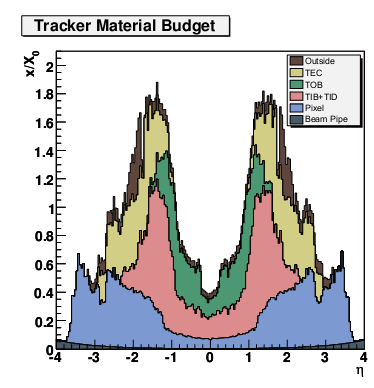
\includegraphics[width=0.6\textwidth]{plots/CMS/TrackerMaterial.png}
\caption{Material budget of the CMS tracking detector in units of radiation length $X_0$ as a function of $\eta$~\cite{CMS}.}
\label{fig:trackerMaterial}
\end{figure} 
\subsection{Electromagnetic calorimeter}
The electromagnetic calorimeter (ECAL) measures the energy of electrons and photons. It uses lead tungstate ($\mathrm{PbWO}_4$) crystals as both absorber and active material. The electromagnetic shower induced by the electron or photon leads to the emission of scintillation light in the crystal, which is measured at the backside of the crystals by avalanche photo diodes (APDs) in the barrel segment of the ECAL and more radiation hard vacuum photo triods (VTPs) in the endcap region. The choice of lead tungstate was driven by the need for a material that is at the same time dense ($\unit{8.28}{\gram\per\centi\cubic\meter}$), has a small Moli\`{e}re radius ($\unit{2.2}{\centi\meter}$), and has a fast response. About 80\% of the scintillation light is emitted within $\unit{25}{\nano\second}$, which is the time between two LHC bunch crossings under design conditions. 
\begin{figure}[htbp]
\centering
  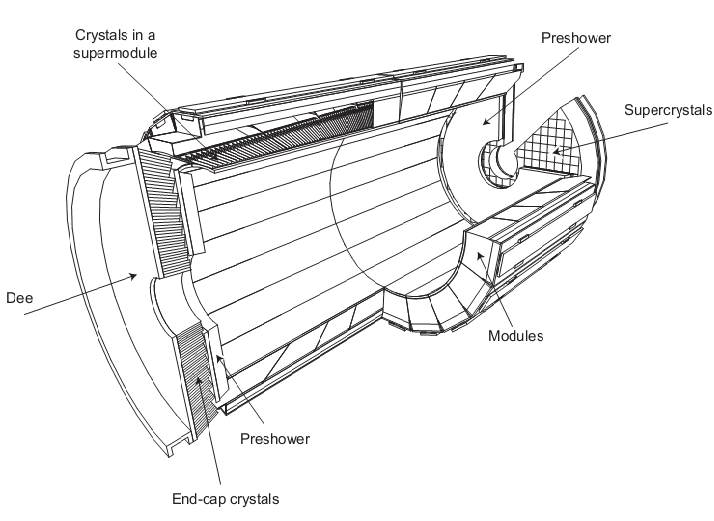
\includegraphics[width=0.6\textwidth]{plots/CMS/ECAL.png}
\caption{Schematic view of the CMS ECAL.}
\label{fig:ECAL}
\end{figure} 
The structure of the ECAL is shown in Figure~\ref{fig:ECAL}. The ECAL barrel (EB) covers the region of $\vert \eta \vert < 1.479$ and consists of 61200 crystals. They have a size of $\unit{2.2\times2.2}{\centi\meter\squared}$ at the front and $\unit{2.6\times2.6}{\centi\meter\squared}$ at the back, with a length of $\unit{23}{\centi\meter}$, corresponding to 25.8 $X_0$. In the ECAL endcaps (EE), consisting of 7324 crystals each, the crystals are slightly larger ($\unit{2.862\times2.862}{\centi\meter\squared}$ to $\unit{3.0\times3.0}{\centi\meter\squared}$) and shorter ($\unit{22}{\centi\meter}$, corresponding to 24.7 $X_0$). The EEs extend the geometric coverage of the ECAL to $\vert \eta \vert = 3.0$. 

In the region of $1.653 < \vert \eta \vert < 2.6$ a preshower detector, consisting of two layers of silicon strips and two layers of lead absorber, is installed to distinguish between prompt photons and those from the decay $\pi^0 \rightarrow \gamma\gamma$. The strips, oriented perpendicular to each other, have a pitch of $\unit{2}{\milli\meter}$, allowing to resolve the two showers of the photons from the $\pi^0$. 

The production of scintillation photons per deposited energy is temperature dependent. Therefore, the ECAL is kept at a temperature of $\unit{18\pm0.05}{\celsius}$, which results in a yield of about 4.5 photons per $\mathrm{MeV}$. 

The typical energy resolution of the ECAL is parametrised as
\begin{equation}
\left(\frac{\sigma}{E}\right)^2 = \left( \frac{2.8\%}{\sqrt{E}}\right)^2 + \left( \frac{0.12}{E} \right)^2 + (0.30\%)^2,
\end{equation}
with three terms describing different sources of uncertainty. The first term includes statistical fluctuations in the production of scintillation light as well as the energy distribution over several crystals. The second term covers such sources of noise as electronic noise or pileup. The constant term accounts for other sources of uncertainties such as calibration errors. The size of the different contributions has been confirmed in test beam measurements~\cite{EGM-10-003}. 
\subsection{Hadron calorimeter}
The hadron calorimeter (HCAL) measures the energy of charged and neutral hadrons. In the barrel region of the detector it is situated between the ECAL and the coil of the solenoid, at radii between $\unit{1.7}{\meter}$ and $\unit{2.95}{\meter}$, limiting the amount of material that can be used in its construction and therefore its ability to contain the hadronic showers. Therefore, additional detectors are placed outside of the volume of the magnet, forming the hadron outer calorimeter (HO). The HCAL barrel (HB) is complemented on each side by a HCAL endcap (HE) and the geometric coverage is extended to high values of $\vert \eta \vert$ by dedicated forward calorimeters (HF). The placement of these subdetectors relative to the other components of CMS is shown in Figure~\ref{fig:HCAL}.
\begin{figure}[htbp]
\centering
  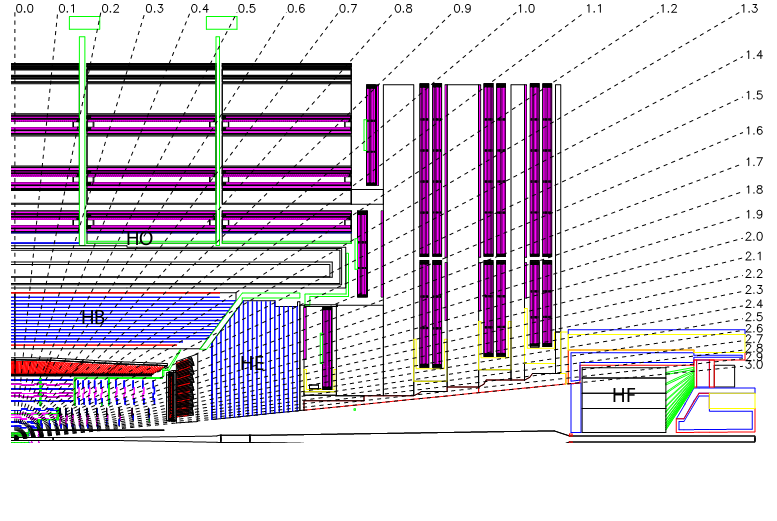
\includegraphics[width=0.6\textwidth]{plots/CMS/HCAL.png}
\caption{Schematic view of the CMS HCAL~\cite{CMS}.}
\label{fig:HCAL}
\end{figure} 
\subsubsection*{HCAL barrel and outer detectors (HB and HO)}  
The HB covers the geometric region $\vert \eta \vert \leq 1.3$. It is constructed as a sandwich calorimeter, consisting of plastic scintillator as the active material. For the absorber material, the fourteen inner layers of the HB are made from brass, while steel is used for the front and back plates of the HB to increase the stability of the construction. The scintillator is divided into 144 segments in $\phi$ and 32 segments in $\eta$, resulting in a spatial granularity of 0.087 in both $\eta$ and $\phi$. The scintillation light produced in the active material is transported to hybrid photo diodes using scintillating fibres. As all layers of one tower in $\eta$ and $\phi$ are read out by the same photo diode, there is no segmentation in the readout in $r$, except for the two towers closest to the HE on each side. The material of the ECAL in front of the HB corresponds to about 1.1 interaction length $\lambda_i$. The absorber material of the HB itself amounts to only 5.82 $\lambda_i$ at $\eta = 0$, which increases to 10.6 $\lambda_i$ at $\vert \eta \vert = 1.3$. To measure the energy of jets not contained in the HB, the HO is placed outside the vacuum containment of the solenoid. It consists of one additional layer of scintillator, with the magnet acting as absorber, except for the most central part of the detector, where one additional layer of steel absorber and scintillator are installed. Hereby the material budget of the HCAL is increased to at least 10 $\lambda_i$ over the whole barrel region.

\subsubsection*{HCAL endcaps (HE)}
The HE extends the geometric coverage of the HCAL up to $\vert\eta\vert =3.0$, coinciding with the coverage of the EEs. It is constructed from the same combination of brass absorber and plastic scintillator as the HB and for the region $1.3 \leq \vert\eta\vert \leq 1.6$ also retains the $\Delta\eta \times \Delta \phi = 0.087\times 0.087$ granularity in $\eta$ and $\phi$. For $\vert\eta\vert \geq 1.6$ the segmentation is coarser, resulting a granularity of $\Delta\eta \times \Delta \phi \approx 0.17\times0.17$. This structure again corresponds to about 10 $\lambda_i$. The longitudinal segmentation of the readout of the towers differs based on the location of the tower. The two towers closest to the beam line are read out in three segments, while most others are divided into two segments. The two towers overlapping with HB are read out without longitudinal segmentation. Multipixel hybrid photo diodes have been chosen for the readout due to their low sensitivity to magnetic fields.
\subsubsection*{Hadron forward calorimeter (HF)}
Of all subdetectors of CMS, the HF covers the highest values of $\vert\eta\vert$, extending up to $\vert\eta\vert = 5.2$. This close to the beam pipe radiation hardness is the key feature of the design, as nearly 90\% of the energy deposited in the detector as the result of a proton-proton interaction is allotted to the HF. It is constructed as two $\unit{3.5}{\meter}$ long cylinders with a radius of $\unit{1.3}{\meter}$, located at $\vert z \vert = \unit{11.2}{\meter}$. The first $\unit{1.65}{\meter}$ consist of plates of steel with a thickness of $\unit{5}{\milli\meter}$, again corresponding to about 10 $\lambda_i$. The active components are quartz fibres, which are inserted into grooves in the steel plates. The particles created in showers in the absorber emit Cherenkov radiation in the fibres, which is detected by photomultiplier tubes at their end. As the Cherenkov threshold is lowest for electrons, at $\unit{190}{\kilo\electronvolt}$, the HF is more sensitive towards electromagnetic than hadronic showers. To separate these two kinds of showers, half of the fibres start only at a depth of $\unit{22}{\centi\meter}$ inside the absorber. As electromagnetic showers develop faster, they deposit most of their energy before this point, which distinguishes them from hadronic showers. 	     
\subsection{Muon system} 
Muons are in general not stopped by any of the subdetectors of the CMS detector inside the solenoid. Therefore, they can be measured with high precision in a clean environment outside of it. Hence, the muon detectors are placed inside the return yoke of the magnet, both for the muon barrel (MB), covering up to $\vert\eta\vert = 1.2$ and the muon endcap (ME) detectors, placed between $\vert\eta\vert = 0.9$ and $\vert\eta\vert = 2.4$. Being placed so far away from the interaction point, the muon detectors have to cover a large area, which requires them to be rather inexpensive compared to other technologies used in the construction of CMS. Three different types of gaseous detectors are used to provide at the same time identification, \pt measurement, and triggering for muons. In the barrel region, drift tubes (DT) are used as the main muon detectors, whereas in the endcaps cathode strip chambers (CSC) are used which are faster and better equipped to deal with the larger and inhomogeneous magnetic field in this region of the detector. To provide a very fast muon tagging for the trigger, resistive plate chambers (RPC) complement the other two technologies in both the barrel and the endcaps. 
\subsubsection*{Drift tubes (DT)}
In the barrel, there are four layers of muon detectors, called muon stations, of which two are located inside the return yoke of the magnet and the other two are located between the solenoid and the yoke and outside the yoke, respectively. The muon stations consist of eight to twelve muon chambers, which are made of two or three superlayers of DTs. The superlayers in turn consist of four layers of DTs. The first three muon stations contain chambers with superlayers measuring either in the $r-\phi$ plane or measuring the $z$ coordinate. In the last muon station only the superlayers measuring in $r-\phi$ are present. The DTs in each layer are offset by half of the width of a tube with respect to the next one to avoid dead spots in the geometric coverage. The DT system consists of about 172000 sensitive wires. The drift tubes are filled with a mixture of 85\% Ar and 15\% $\text{CO}_2$, and their structure is shown in Figure~\ref{fig:DT} The $r\phi$ resolution of a single DT is about $\unit{250}{\micro\meter}$, so that one muon chamber, which contains two superlayers with four DTs measuring in the $r-\phi$ plane each, reaches a precision of $\unit{100}{\micro\meter}$.
\begin{figure}[htbp]
\centering
  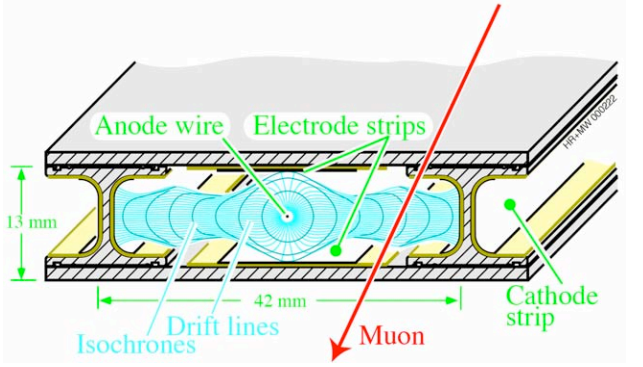
\includegraphics[width=0.6\textwidth]{plots/CMS/DT.png}
\caption{Schematic view of one drift tube~\cite{CMS}.}
\label{fig:DT}
\end{figure}  
\subsubsection*{Cathode strip chambers (CSC)}
The CSC are multiwire proportional chambers, consisting of six planes of anode wires interleaved with seven panels of cathode strips. The chambers have trapezoidal shapes and are arranged in four discs around the beam axis, each further segmented into two or three rings. The cathode strips measure the $\phi$ coordinate while the anode wires measure the radial coordinate. Figure~\ref{fig:CSC} shows the structure of one chamber on the left side and the creation of a signal due to an amplification of the initial ionisation in an avalanche close to the anode wire on the right side. 
\begin{figure}[htbp]
\centering
  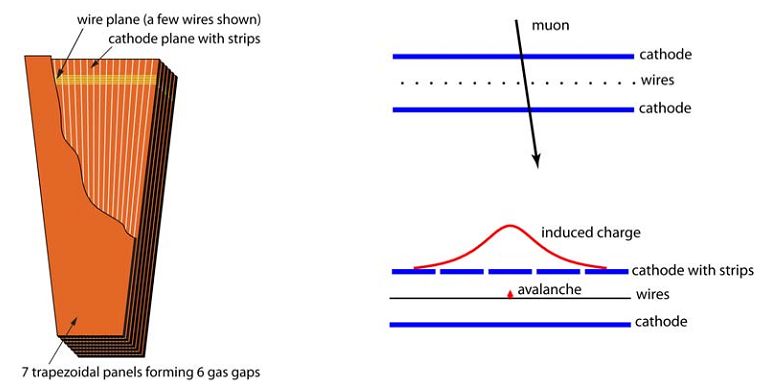
\includegraphics[width=0.85\textwidth]{plots/CMS/CSC.png}
\caption{Schematic view of one CSC (left) and the creation of a signal (right)~\cite{CMS}.}
\label{fig:CSC}
\end{figure}  
\subsubsection*{Resistive plate chambers (RPC)}
The RPCs consist of three layers of bakelite, which form two small gas filled gaps and between which high voltage is applied. The amplification of the initial signal is very fast in this configuration, with drift times of about $\unit{5}{\nano\second}$. Therefore, this technology is well suited to associate muon candidates to the LHC bunch crossings. In the barrel region six layers of RPCs are installed, while three layers are used in the endcaps for $\vert\eta\vert \leq 1.6$.
\subsubsection*{Momentum resolution}
The \pt resolution of the muon system alone was expected to be about 10\% for muons with \pt up to $\unit{200}{\giga\electronvolt}$. Combined with the information from the inner tracking system, a resolution of about 1\% was expected to be achieved in the central region of $\vert\eta\vert \leq 0.8$ for a \pt of $\unit{10}{\giga\electronvolt}$, increasing to about 2\% for a \pt of $\unit{200}{\giga\electronvolt}$.

The \pt resolution for muons has been measured using data collected in 2010~\cite{MUO-10-004}. Using the muon system alone, resolutions better than 10\% have been found for the barrel region for muons with \pt $> \unit{15}{\giga\electronvolt}$. The muon resolution improves when combining the information from the muon system with those from the inner tracking system. The precision of the tracking system dominates for a wide \pt range and averaging over $\eta$ and $\phi$ resolutions of 1.8$\pm$0.3(stat.)\% at $\unit{\pt = 30}{\giga\electronvolt}$ to 2.3$\pm$0.3(stat.)\% at $\unit{\pt = 50}{\giga\electronvolt}$ have been achieved.
